%%%%%%%%%%%%%%%%%%%%%%%%%%%%%%%%%%%%%%%%%%%%%%
%                insertmeeting
% 1) Title (something creative & funny?)
% 2) Date (MM/DD/YYYY)
% 3) Location (ex. Hagerty High School)
% 4) People/Committees Present 
% 5) Picture 
% 6) Start Time & Stop Time (ex. 12:30AM to 4:30PM)
%%%%%%%%%%%%%%%%%%%%%%%%%%%%%%%%%%%%%%%%%%%%%%
\insertmeeting 
	{Material Mania} 
	{02/19/22} 
	{Hagerty High School}
	{James, Jensen, Nathan, Ritam}
	{Images/RobotPics/robot.jpg}
	{2:30 - 4:30}
	
\hhscommittee{Software}
\noindent\hfil\rule{\textwidth}{.4pt}\hfil
\subsubsection*{Goals}
\begin{itemize}
    \item Take apart old arm supports and replace them with carbon fiber sides
	\item Test for potential radio signal issues from carbon fiber plates


\end{itemize} 

\noindent\hfil\rule{\textwidth}{.4pt}\hfil

\subsubsection*{Accomplishments}
Recently, we talked to a materials scientist who warned us of carbon fibers' ability to block radio signals, which the robot uses in the form of WiFi to connect to our driver station, due to its conductive properties. Although this was a potential risk, he added, there was a low chance that the thickness of carbon fiber that we are using will have any significance on the connection. With this new information, we put a control hub inside the carbon fiber then connected it to a motor. We then downloaded code that would make the motor spin with an input from a controller, which will allow us to see if there is any noticeable delay in controls with the carbon fiber. Thankfully, there seemed to be no delay and our ping was totally normal. Despite this win, we still need to test to see if the robot, with more things running at once, will work without delay.
But before we can test that, we need to actually attach the carbon fiber sides, which first means removing the old REV extrusions which held up the arms before we made the carbon fiber. We were able to quickly detach the structure, making sure to keep it intact just in case we had any catastrophic connection issues after we tested. Taking the arm off of the old arm supports, we reattached it to the carbon fiber sides and checked to make sure there were no interferences between the parts. We then added some threaded inserts into the polycarbonate drivetrain using a soldering iron, which heats up the plastic enough for the brass inserts to slide in. Using these threaded inserts, we were able to attach the carbon fiber sides successfully onto the robot (Figure \ref{fig:021922_1}). 
Pleased with our work, we moved onto testing the robot by driving it around in teleop to make sure everything was in order. Not noticing any connection issues, we were feeling more confident about this design every second and are becoming more excited to showcase it at leagues. As an added benefit, we noticed that the light weight of the carbon fiber and the new location of the core hex motor and battery, both of which are located lower on the robot than before,  made the robot smoother to steer and less likely to tip over. Finally in a complete state, we are ready to hand the robot over to software to create our magical autonomous!


\begin{figure}[htp]
\centering
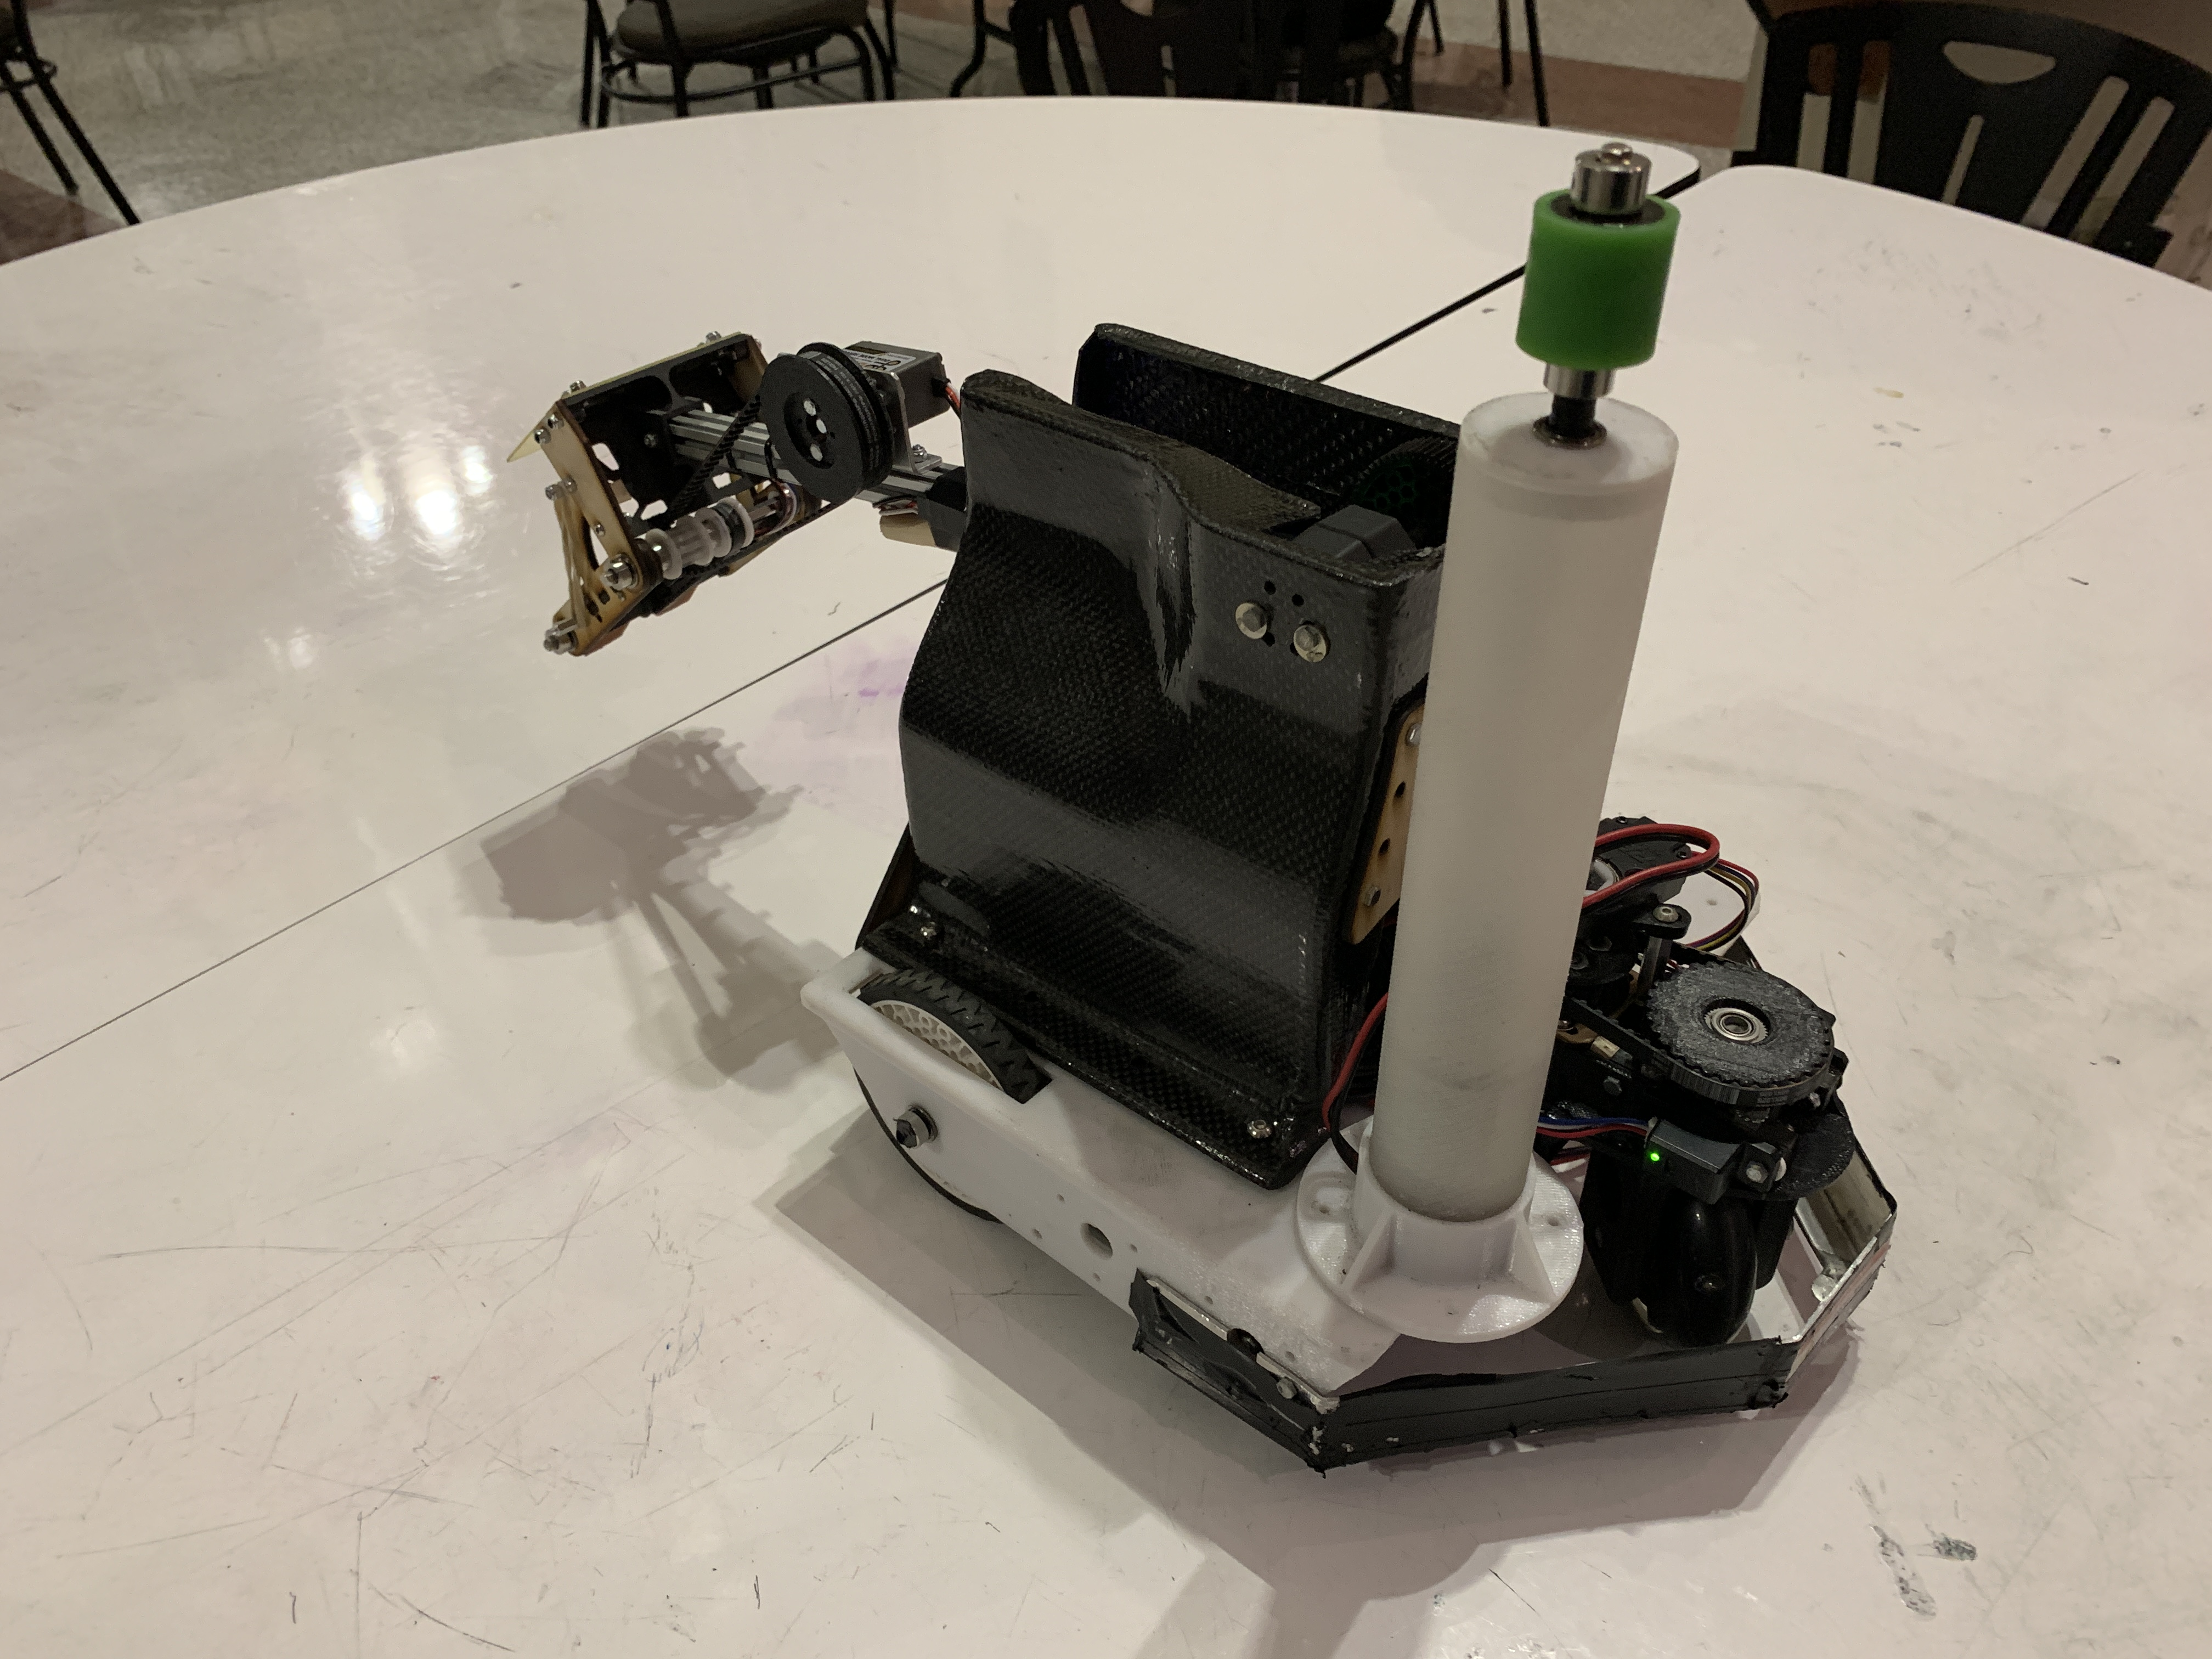
\includegraphics[width=0.95\textwidth, angle=0]{Meetings/February/02-19-22/2-19-22_Hardware_Figure1 - Nathan Forrer.JPG}
\caption{Attaching the carbon fiber sides using threaded inserts}
\label{fig:021922_1}
\end{figure}


\whatsnext{
\begin{itemize}
    \item Let software take over to create an awesome autonomous!
\end{itemize} 
}

